\documentclass[11pt]{article}
\usepackage{graphicx}
\usepackage{subcaption}
\usepackage{hyperref}
\usepackage[parfill]{parskip}
\title{CITS2200 Project Report}
\author{Robin Markwitz (21968594) \& Frederick Subere Albawy (21960842)}
\begin{document}
	\maketitle
	\section{Graphs}
	\subsection{Introduction}
	A graph is a structure that consists of vertices and edges. An edge connects two vertices together.
	Graphs can be either (a) undirected or (b) directed. A graph is directed when an edge connecting two vertices is only in one direction - this is indicated by the use of an arrow. In an undirected graph, an edge denotes a connection in both directions - no arrows are used.
	\begin{figure}[h!]
		\centering
		\begin{subfigure}{.5\textwidth}
			\centering
			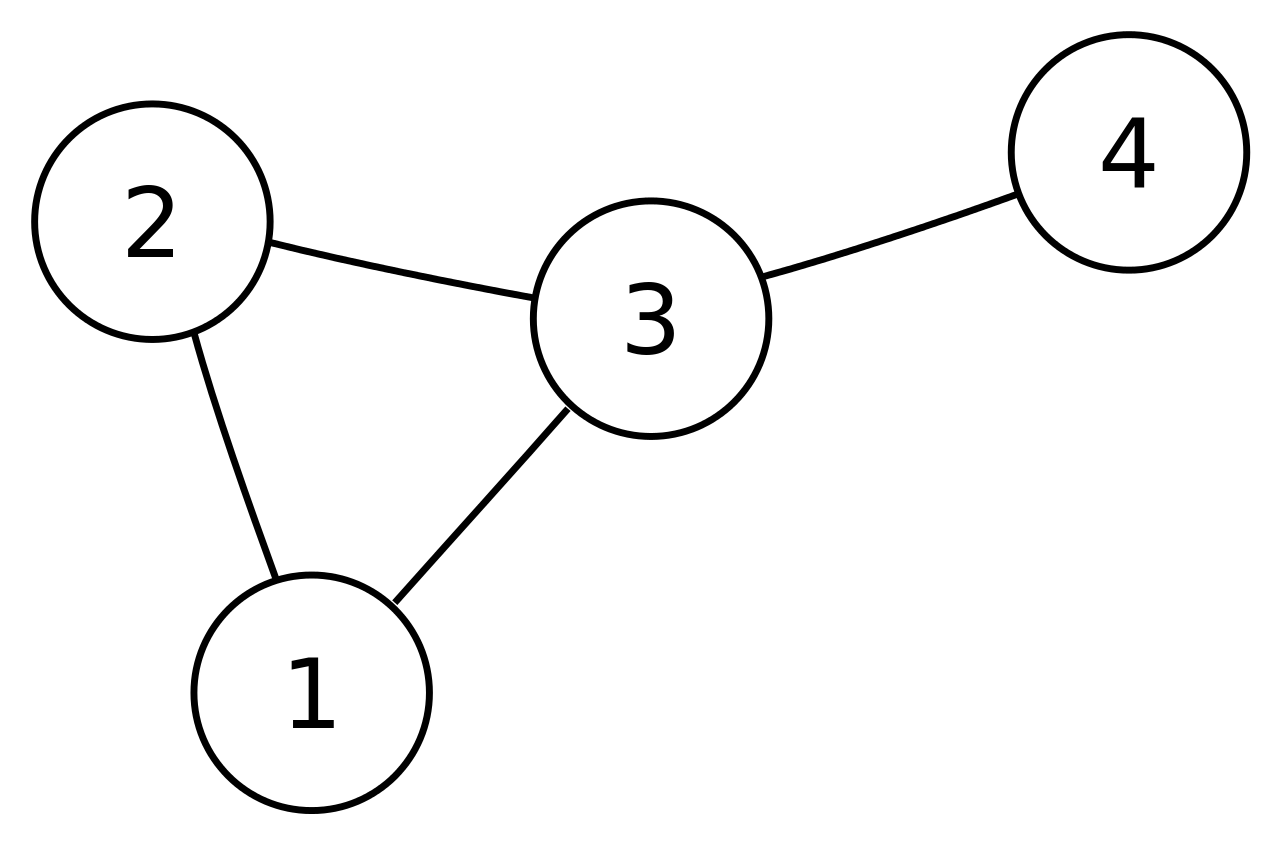
\includegraphics[width=.4\linewidth]{images/Undirected_graph.jpg}
			\caption{An undirected graph.}
			\label{fig:sub1}
		\end{subfigure}%
		\begin{subfigure}{.5\textwidth}
			\centering
			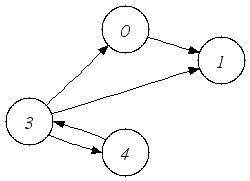
\includegraphics[width=.4\linewidth]{images/directedGraph.jpg}
			\caption{A directed graph.}
			\label{fig:sub2}
		\end{subfigure}
		\label{fig:test}
	\end{figure}
	\\
	A graph can also be weighted (see below). This means that there is a number on the edge that signifies its weight, or value.
	\begin{figure}[h!]
		\centering
		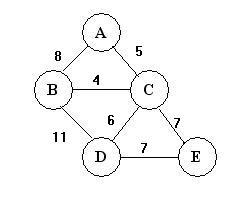
\includegraphics[width=50mm,scale=0.5]{images/weighted_graph.jpg}
	\end{figure}
	\newpage
	\subsection{The Wikipedia Graph}
	In our project we were assigned to analyze subsets of the Wikipedia graph and to find properties of these subgraphs. The vertices of the graph denote pages and an edge exists between two pages just when there is a link connecting one page to the other. It is easy to see that a subset of the Wikipedia graph, and the Wikipedia graph itself, is directed - as there may be a link between page A and B, but there must not necessarily be a link between page B and A.
	\newline
	It is also easy to see that the Wikipedia graph is unweighted. There is no discernible difference between any two links and thus there is no need to assign a weight to any edges. Therefore the Wikipedia graph is a directed and unweighted graph.
	\section{Project Outline}
	\subsection{Details}
	We have written/implemented many different graph algorithms to discover features of subsets of the Wikipedia graph. The \texttt{CITS2200Project} interface was used. We included two private classes along with our main \texttt{WikiGraphAnalyzer} class. The following problems were to be solved: \cite{amitava}
	\begin{enumerate}
		\item Write a method that, given a pair of pages, returns the minimum number of links you must follow to get from the first page to the second.
		\item Write a method that finds a Hamiltonian path in a Wikipedia page graph. A Hamiltonian path is any path in some graph that visits every vertex exactly once. This method will never be called for graphs with more than 20 pages.
		\item Write a method that finds every ‘strongly connected component’ of pages. A strongly connected component is a set of vertices such that there is a path between every ordered pair of vertices in the strongly connected component.
		\newpage
		\item Write a method that finds all the centers of the Wikipedia page graph. A vertex is considered to be the center of a graph if the maximum shortest path from that vertex to any other vertex is the minimum possible. 
	\end{enumerate}
	The algorithms we used to solve these problems will be introduced and explained in the following section - along with some performance analysis and their sources.
	\subsection{Our implementation of the Wikipedia graph}
	The data structure that we decided to use to hold the set of pages and links of the Wikipedia graph was the adjacency list - specifically implemented in Java as an \texttt{ArrayList} of \texttt{ArrayLists}. This allows us to iterate easily and also makes reversing the graph efficient. We chose to use \texttt{ArrayList} due to better performance when adding to the end of the list in comparison to \texttt{LinkedList}, which was the other option. We also decided to use a \texttt{PriorityQueue} to assist with Problem 1, and various other data structures in other methods. In addition to this, we implemented two inner classes:
	\begin{itemize}
		\item A class called \texttt{Node} which holds a \texttt{String} and an \texttt{int} variable. This is necessary for our use of \texttt{java.util.PriorityQueue}.
		\item A class called \texttt{NodeComparator}, which compares two \texttt{Objects} from the class \texttt{Node} and applies an ordering on the two. This ordering is necessary such that a \texttt{PriorityQueue<Node>} has the context to order \texttt{Nodes} in a certain way.
	\end{itemize}
	
	\section{Algorithms used}
	\subsection{Problem 1}
	This problem is also known as the shortest path problem, as finding the minimum amount of links between two pages is analogous to finding the shortest path between two vertices. We have implemented Dijkstra's algorithm to find the shortest path between one page (or vertex) and another. The pseudocode can be found here: \cite{dijkstra}
	\newpage
	\begin{figure}[h!]
		\centering
		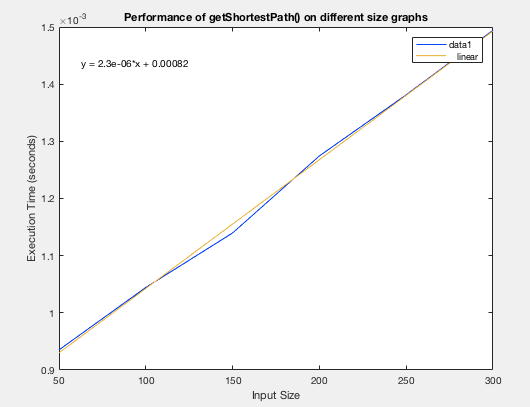
\includegraphics[width=\linewidth]{images/dijkstra.jpg}
	\end{figure}
	Q denotes a priority queue, which takes \texttt{Node} objects. The array dist is the distance from the given vertex to all other vertices in the graph - however as we only are interested in a given vertex, we return only that vertex's shortest path instead of other shortest paths to other nodes.
	\\
	We also decided to neglect the array prev, which denotes the predecessors of vertices, as it was not relevant for this implementation of the algorithm.
	\subsubsection{Complexity}
	The complexity of Dijkstra's algorithm is \(O(|E|\log|V|)\) \\ where \(E = \{e_1,e_2,e_3,...,e_n\}\) is the set of all edges in the graph and \(V = \{v_1,v_2,v_3,...,v_n\}\) is the set of all vertices in the graph.
	\\
	For an unweighted directed graph this is the optimum algorithm to use as it is efficient and reliable.
	\subsubsection{Performance Analysis}
	Dijkstra's algorithm was tested on a number of different graphs with the same sparseness. Only the helper method getShortestPathArray was tested, as this contains the implementation of Dijkstra's algorithm and avoids the constant time operations of calling the helper method and extracting the required result from the array.
	\newline
	The performance of the algorithm with respect to the size of the input in vertices is best modeled with a linear fit. The complexity of the algorithm is \(O(|E|\log|V|)\). In a maximally dense graph with edges between all pairs of vertices (\(|E| = |V|^2\)), this would result in a complexity somewhere between quadratic and cubic, whereas in a sparse graph where \(|E| = |V|\), complexity would be between quadratic and linear. The linear result obtained in this case suggests that the graph is of low density.
	\begin{figure}[h!]
 		\centering
 		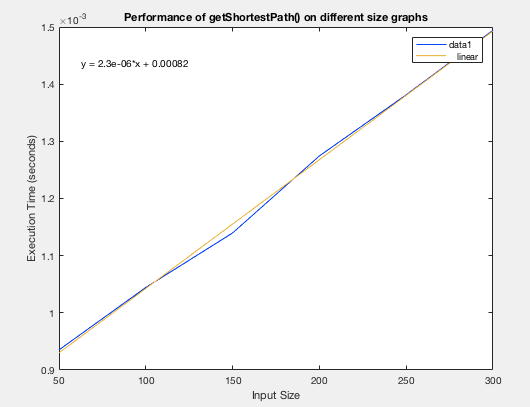
\includegraphics[width=100mm,scale=0.5]{images/dijkstra.png}
 	\end{figure}

	\subsection{Problem 2 - Hamiltonian path}
	A Hamiltonian path, also called a Hamiltonian cycle, is a path in a graph that visits each vertex once and only once. A Hamiltonian cycle may not necessarily exist in every graph, though a graph may have one, or more than one, Hamiltonian cycle. Though the Hamiltonian path can be found via a brute force method, we have elected to use an algorithm that utilizes dynamic programming techniques to find the Hamiltonian path through analyzing each element of the power set of \(V\). The algorithm used was the Bellman-Held-Karp algorithm, which can be stated in pseudocode: \cite{hamilton} \newpage 
	 \begin{figure}[h!]
	 	\centering
	 	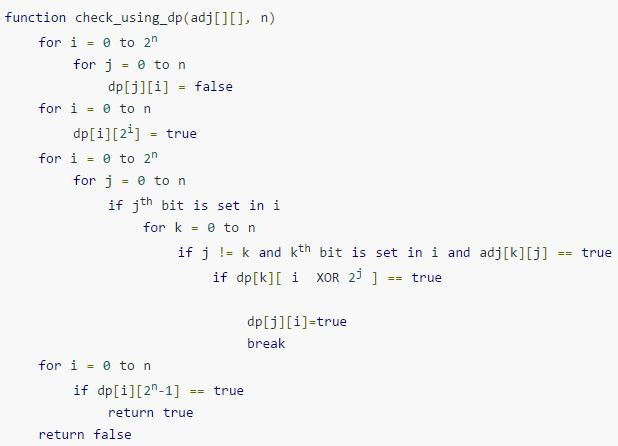
\includegraphics[width=100mm,scale=0.5]{images/Capture.jpg}
	 \end{figure}
 	This algorithm works on the following idea: For a graph \(G = (V,E)\), take an arbitrary subset \(S \subseteq V\). For a given vertex \(v \in S\), is there a path starting at some other arbitrary vertex \(w \in S\) that goes through all \(S = \{s_1,s_2,s_3,...\}\), ending at \(v\)? As with all other dynamic programming problems, a base case - there is only one node in the arbitrary subset \(S\) - is established, and the answers that this gives are used to compute the next solution, until the complete solution is found. As the largest subset of \(V\) is \(V\) itself, the final column in the previously initialized boolean array will be the truth values of the existence of the full Hamiltonian cycle. If a Hamiltonian cycle does exist, then backtracking is used to find this cycle. 
 	\subsubsection{Complexity}
 	The main loop runs \(1<<n\) times, where \(n = |V|\), and \(<<\) is the left bit shift operator. \(n\) bit shifted left 1 position is equivalent to \(2^n\), and thus it runs \(2^n\) times. The two inner loops within this outer loop both run \(n\) times, so the overall complexity can be stated as \(O(2^n n^2)\).
 	\newpage
 	\subsubsection{Performance Analysis}
 	\begin{figure}[h!]
 		\centering
 		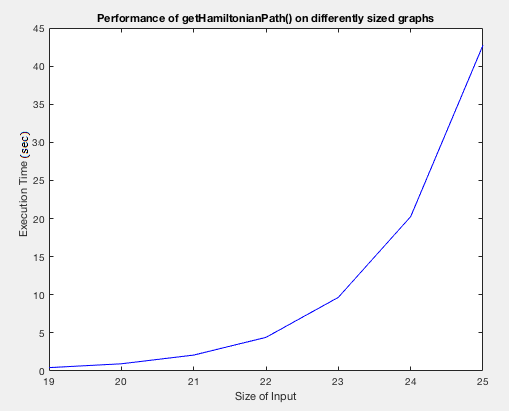
\includegraphics[width=100mm,scale=0.5]{images/hamiltonian_performance.png}
 	\end{figure}
 	The algorithm was tested on 7 different graphs - all with similar sparseness, generated via an automated text file writer class in Java. It was tested 10 times on each graph and then the arithmetic mean was taken of these values, for each graph. These data were recorded in MS Excel before then being read into MATLAB to be plotted. \\
 	It can be seen that the time taken to execute the algorithm increases exponentially as the size of input increases. This would be consistent with the theoretical complexity of the algorithm, which is non-polynomial in nature.
	Since the complexity is \(O(2^n n^2)\), graphs of different sparseness should not differ in performance.
	\subsection{Problem 3 - Strongly connected components of a graph}
	If we let \(G = (V,E)\) be a directed graph, then two nodes \(u,v \in V\) are strongly connected just when \(v\) is reachable from \(u\) and \(u\) is reachable from \(v\).
	\newline
	A strongly connected component of \(G\) is a set \(C\subseteq V\) such that:
	\begin{itemize}
		\item \(C \neq \emptyset\).
		\item \(\forall u,v \in C\), \(u\) and \(v\) are strongly connected.
		\item \(\forall u \in C\) and \(\forall v \in (V \setminus C)\), \(u\) and \(v\) are not strongly connected. \cite{stanford}
	\end{itemize}

	For example, consider this graph:
	\begin{figure}[h!]
		\centering
		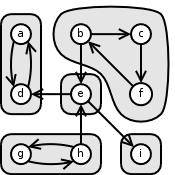
\includegraphics[width=50mm,scale=0.5]{images/SCC.jpg}
	\end{figure}
	\newline
	There are 5 strongly connected components in this graph - namely \(\{a,d\}\), \(\{e\}\), \(\{b,c,f\}\), \(\{g,h\}\) and \(\{i\}\). These components are strongly connected because for each element in each component, the only elements that can be reached, that also reach it, are all the other elements in the component. 
	The algorithm that we used was Kosaraju's algorithm: \cite{scc}
	\begin{figure}[h!]
		\centering
		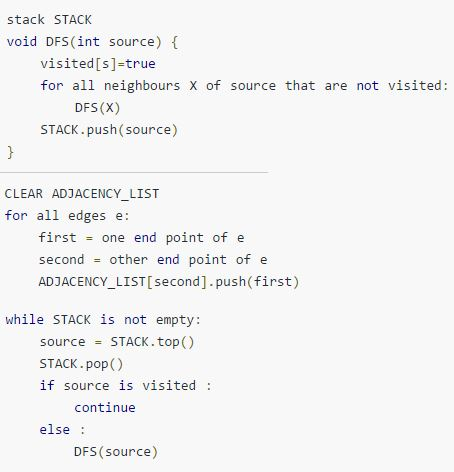
\includegraphics[width=80mm,scale=0.5]{images/kosaraju.jpg}
	\end{figure}
	\newline
	The idea of this algorithm is to perform one depth-first search (DFS) on the graph and to add each newly found vertex to a stack. Then the graph is reversed, and then a second pass of DFS is performed on the reversed graph, taking the vertices that are on top of the stack and popping until the stack is empty. This works because if vertices are visited in one direction and then visited in the other, they must be strongly connected to each other. The stack ensures that the vertex with the longest finishing time in the forward DFS is visited first in the reverse DFS.
	\subsubsection{Complexity}
	The worst case complexity is \(O(|E| + |V|)\), where \(E = \{e_1,e_2,e_3,...,e_n\}\) is the set of all edges in the graph and \(V = \{v_1,v_2,v_3,...,v_n\}\) is the set of all vertices in the graph. This is because in the worst case, this algorithm will visit every single edge and every single vertex in the graph.
	\subsubsection{Performance Analysis}
	\begin{figure}[h!]
		\centering
		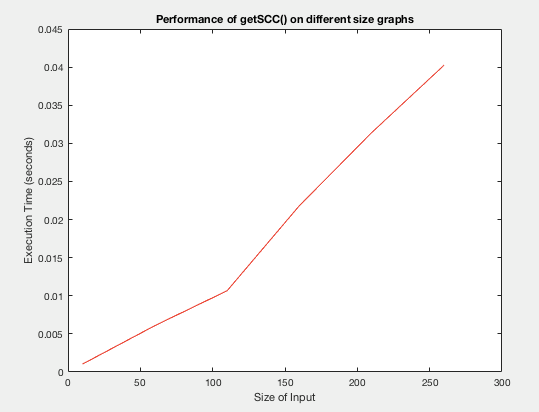
\includegraphics[width=100mm,scale=0.5]{images/strongconnect.png}
	\end{figure}
	Due to the relative sparsity of the randomly generated graphs, this algorithm is linear in performance. Though theoretically it may reach \(O(|V|^2 + |V|)\) in the worst case (where there is an edge between every possible node) it performs linearly in the average case. It does not deteriorate significantly as the size of the input increases and thus can be relied on even for very large graphs.
	\subsection{Problem 4 - Get centers of a graph}
	The center vertices of a graph \(G = (V,E)\) are contained in a set \(C \subseteq V\), where \(c_i \in C\) are the vertices where the maximum distance from \(c_i\) to any other vertex \(v \in V\) is the smallest possible. This problem can also be worded in the following way: \\
	Let \(\epsilon (v) = \max\limits_{u \in V} \ d(v,u)\) where \(d(v,u)\) is the shortest path from a vertex \(v\) to a vertex \(u\). This is often called the eccentricity of a vertex. Then the radius of a graph \(G\) can be written as \(rad(G) = \min\limits_{v \in V} \epsilon (v) \), and the centers of a graph can simply be expressed as the set of vertices whose eccentricities are equal to the radius of the graph. \cite{centers}
	\\
	\\
	The algorithm that was used to calculate this performed that exact task:
		\begin{figure}[h!]
		\centering
		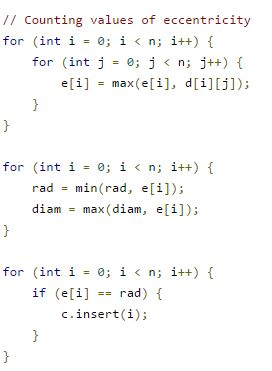
\includegraphics[width=50mm,scale=0.5]{images/centers.jpg}
		\end{figure}
	\newline
	A matrix of all-pair shortest paths was found, and then eccentricities and radii were found to find all the vertices that were centers of the graph, as defined earlier. 
	\subsubsection{Complexity} 
	Calculating the all-pair shortest path matrix of a graph \(G\) requires \(|V|\) calls of Dijkstra's algorithm, which has a complexity of \(O(|E|\log|V|)\). This term dominates in the complexity analysis of this algorithm and therefore it can be concluded that the complexity of this algorithm is \(O(|V||E|\log|V|)\).
	\subsubsection{Performance Analysis}
	\begin{figure}[h!]
		\centering
		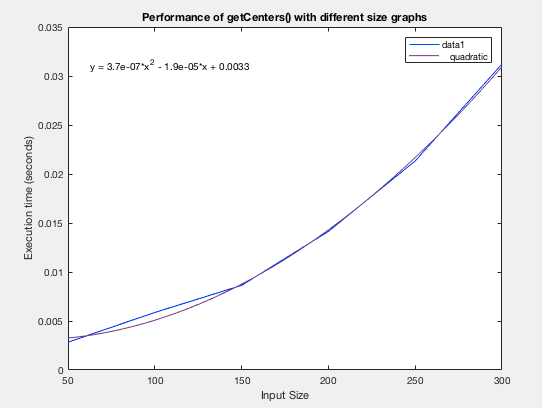
\includegraphics[width=100mm,scale=0.5]{images/centres.png}
	\end{figure}
	The complexity is \(O(|V||E|\log|V|)\), as the algorithm requires \(|V|\) calls of Dijkstra's algorithm, so given that the performance of Dijkstra's algorithm was found to be linear for this particular graph in section 3.1.2, quadratic performance for this algorithm would be expected. For more dense graphs than this one, the performance would be cubic, because in the worst case, \(E = |V|^2\), and thus your overall complexity would be \(O(|V|^3 \log V)\).
	\newpage
	\begin{thebibliography}{9}
		\bibitem{amitava}
		Datta, A. \textit{CITS2200 - Data Structures And Algorithms.} \\\url{http://teaching.csse.uwa.edu.au/units/CITS2200/Labs/project-2017/project-2017.html}. \\Last accessed 5/21/2017.
		\bibitem{dijkstra}
		Wikipedia Contributors. \textit{Wikipedia, the free encylopedia.} \\\url{https://en.wikipedia.org/wiki/Dijkstra\%27s\_algorithm}.
		\\Last accessed 6/3/2017.
		\bibitem{hamilton}
		Jaimini, V. \textit{HackerEarth.} \\\url{https://www.hackerearth.com/practice/algorithms/graphs/hamiltonian-path/tutorial/}. \\Last accessed 6/2/2017.
		\bibitem{stanford}
		Stanford University. \textit{Stanford University.} \\\url{https://web.stanford.edu/class/archive/cs/cs161/cs161.1138/lectures/04/Small04.pdf}. \\Last accessed 6/1/2017.
		\bibitem{scc}
		Vikram, R. \textit{HackerEarth.} \\\url{https://www.hackerearth.com/practice/algorithms/graphs/strongly-connected-components/tutorial/}
		\\Last accessed 6/3/2017.
		\bibitem{centers}
		Kassenov, B. \textit{Codeforces.} \\\url{codeforces.com/blog/entry/17974}
		\\Last accessed 5/31/2017.
		
		
		
	\end{thebibliography}	
\end{document}